% Options for packages loaded elsewhere
\PassOptionsToPackage{unicode}{hyperref}
\PassOptionsToPackage{hyphens}{url}
\PassOptionsToPackage{dvipsnames,svgnames,x11names}{xcolor}
%
\documentclass[
  letterpaper,
  DIV=11,
  numbers=noendperiod]{scrartcl}

\usepackage{amsmath,amssymb}
\usepackage{iftex}
\ifPDFTeX
  \usepackage[T1]{fontenc}
  \usepackage[utf8]{inputenc}
  \usepackage{textcomp} % provide euro and other symbols
\else % if luatex or xetex
  \usepackage{unicode-math}
  \defaultfontfeatures{Scale=MatchLowercase}
  \defaultfontfeatures[\rmfamily]{Ligatures=TeX,Scale=1}
\fi
\usepackage{lmodern}
\ifPDFTeX\else  
    % xetex/luatex font selection
\fi
% Use upquote if available, for straight quotes in verbatim environments
\IfFileExists{upquote.sty}{\usepackage{upquote}}{}
\IfFileExists{microtype.sty}{% use microtype if available
  \usepackage[]{microtype}
  \UseMicrotypeSet[protrusion]{basicmath} % disable protrusion for tt fonts
}{}
\makeatletter
\@ifundefined{KOMAClassName}{% if non-KOMA class
  \IfFileExists{parskip.sty}{%
    \usepackage{parskip}
  }{% else
    \setlength{\parindent}{0pt}
    \setlength{\parskip}{6pt plus 2pt minus 1pt}}
}{% if KOMA class
  \KOMAoptions{parskip=half}}
\makeatother
\usepackage{xcolor}
\setlength{\emergencystretch}{3em} % prevent overfull lines
\setcounter{secnumdepth}{-\maxdimen} % remove section numbering
% Make \paragraph and \subparagraph free-standing
\ifx\paragraph\undefined\else
  \let\oldparagraph\paragraph
  \renewcommand{\paragraph}[1]{\oldparagraph{#1}\mbox{}}
\fi
\ifx\subparagraph\undefined\else
  \let\oldsubparagraph\subparagraph
  \renewcommand{\subparagraph}[1]{\oldsubparagraph{#1}\mbox{}}
\fi


\providecommand{\tightlist}{%
  \setlength{\itemsep}{0pt}\setlength{\parskip}{0pt}}\usepackage{longtable,booktabs,array}
\usepackage{calc} % for calculating minipage widths
% Correct order of tables after \paragraph or \subparagraph
\usepackage{etoolbox}
\makeatletter
\patchcmd\longtable{\par}{\if@noskipsec\mbox{}\fi\par}{}{}
\makeatother
% Allow footnotes in longtable head/foot
\IfFileExists{footnotehyper.sty}{\usepackage{footnotehyper}}{\usepackage{footnote}}
\makesavenoteenv{longtable}
\usepackage{graphicx}
\makeatletter
\def\maxwidth{\ifdim\Gin@nat@width>\linewidth\linewidth\else\Gin@nat@width\fi}
\def\maxheight{\ifdim\Gin@nat@height>\textheight\textheight\else\Gin@nat@height\fi}
\makeatother
% Scale images if necessary, so that they will not overflow the page
% margins by default, and it is still possible to overwrite the defaults
% using explicit options in \includegraphics[width, height, ...]{}
\setkeys{Gin}{width=\maxwidth,height=\maxheight,keepaspectratio}
% Set default figure placement to htbp
\makeatletter
\def\fps@figure{htbp}
\makeatother

\usepackage{booktabs}
\usepackage{longtable}
\usepackage{array}
\usepackage{multirow}
\usepackage{wrapfig}
\usepackage{float}
\usepackage{colortbl}
\usepackage{pdflscape}
\usepackage{tabu}
\usepackage{threeparttable}
\usepackage{threeparttablex}
\usepackage[normalem]{ulem}
\usepackage{makecell}
\usepackage{xcolor}
\usepackage[auth-lg]{authblk}
\KOMAoption{captions}{tableheading}
\makeatletter
\makeatother
\makeatletter
\makeatother
\makeatletter
\@ifpackageloaded{caption}{}{\usepackage{caption}}
\AtBeginDocument{%
\ifdefined\contentsname
  \renewcommand*\contentsname{Table of contents}
\else
  \newcommand\contentsname{Table of contents}
\fi
\ifdefined\listfigurename
  \renewcommand*\listfigurename{List of Figures}
\else
  \newcommand\listfigurename{List of Figures}
\fi
\ifdefined\listtablename
  \renewcommand*\listtablename{List of Tables}
\else
  \newcommand\listtablename{List of Tables}
\fi
\ifdefined\figurename
  \renewcommand*\figurename{Figure}
\else
  \newcommand\figurename{Figure}
\fi
\ifdefined\tablename
  \renewcommand*\tablename{Table}
\else
  \newcommand\tablename{Table}
\fi
}
\@ifpackageloaded{float}{}{\usepackage{float}}
\floatstyle{ruled}
\@ifundefined{c@chapter}{\newfloat{codelisting}{h}{lop}}{\newfloat{codelisting}{h}{lop}[chapter]}
\floatname{codelisting}{Listing}
\newcommand*\listoflistings{\listof{codelisting}{List of Listings}}
\makeatother
\makeatletter
\@ifpackageloaded{caption}{}{\usepackage{caption}}
\@ifpackageloaded{subcaption}{}{\usepackage{subcaption}}
\makeatother
\makeatletter
\@ifpackageloaded{tcolorbox}{}{\usepackage[skins,breakable]{tcolorbox}}
\makeatother
\makeatletter
\@ifundefined{shadecolor}{\definecolor{shadecolor}{rgb}{.97, .97, .97}}
\makeatother
\makeatletter
\makeatother
\makeatletter
\makeatother
\ifLuaTeX
  \usepackage{selnolig}  % disable illegal ligatures
\fi
\IfFileExists{bookmark.sty}{\usepackage{bookmark}}{\usepackage{hyperref}}
\IfFileExists{xurl.sty}{\usepackage{xurl}}{} % add URL line breaks if available
\urlstyle{same} % disable monospaced font for URLs
\hypersetup{
  pdftitle={Trabalho Prático 2},
  pdfauthor={Ana Tércia Freires da Silva -; Gabriel Véras Monteiro - 19/0106794; Gabriela Carneiro de Almeida - 18/0120816},
  colorlinks=true,
  linkcolor={blue},
  filecolor={Maroon},
  citecolor={Blue},
  urlcolor={Blue},
  pdfcreator={LaTeX via pandoc}}

\title{Trabalho Prático 2}
\usepackage{etoolbox}
\makeatletter
\providecommand{\subtitle}[1]{% add subtitle to \maketitle
  \apptocmd{\@title}{\par {\large #1 \par}}{}{}
}
\makeatother
\subtitle{Análise de Séries Temporais - 1/2023}
\author{Ana Tércia Freires da Silva - \and Gabriel Véras Monteiro -
19/0106794 \and Gabriela Carneiro de Almeida - 18/0120816}
\date{}

\begin{document}
\maketitle
\ifdefined\Shaded\renewenvironment{Shaded}{\begin{tcolorbox}[interior hidden, sharp corners, breakable, boxrule=0pt, enhanced, borderline west={3pt}{0pt}{shadecolor}, frame hidden]}{\end{tcolorbox}}\fi

\renewcommand*\contentsname{Table of contents}
{
\hypersetup{linkcolor=}
\setcounter{tocdepth}{3}
\tableofcontents
}
\newpage{}

\hypertarget{introduuxe7uxe3o-suxe9rie-selecionada-caracteruxedsticas-e-decomposiuxe7uxe3o}{%
\section{Introdução: série selecionada, características e
decomposição}\label{introduuxe7uxe3o-suxe9rie-selecionada-caracteruxedsticas-e-decomposiuxe7uxe3o}}

A série temporal escolhida foi a de número \emph{id} correspondente a
1891. De acordo com a definição do próprio pacote, refere-se a
\emph{Pneumatic casings, original equipment}. Foram realizadas medidas
mensais de 1982 a 1992 e o horizonte de previsão requerido é das 18
ocorrências seguintes.

O gráfico da série, com \emph{in} e \emph{out-sample}, é exposto a
seguir.

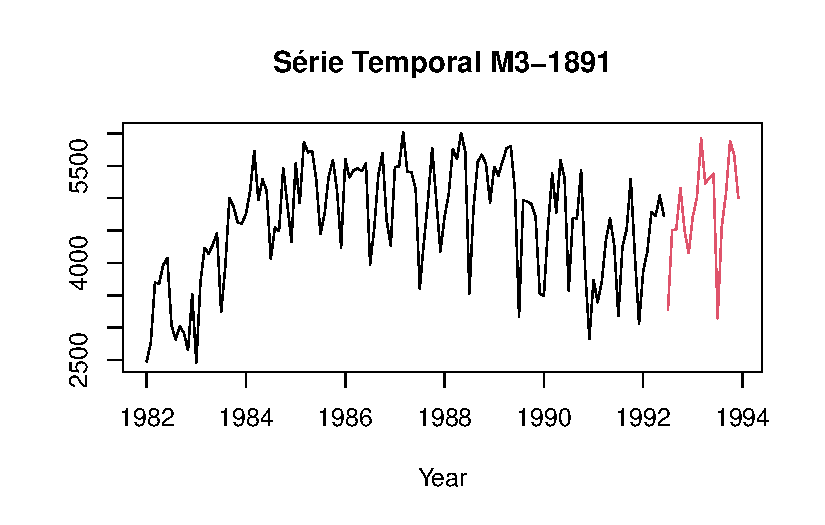
\includegraphics{T2_grupo10_files/figure-pdf/plot-serie-total-1.pdf}

Após visualização inical da série, foi feita sua decomposição via MSTL.
Foram feitas duas decomposições, uma ajustando \emph{lambda = ``auto''}
e \emph{lambda = NULL}, resultando em duas composições muito similares.

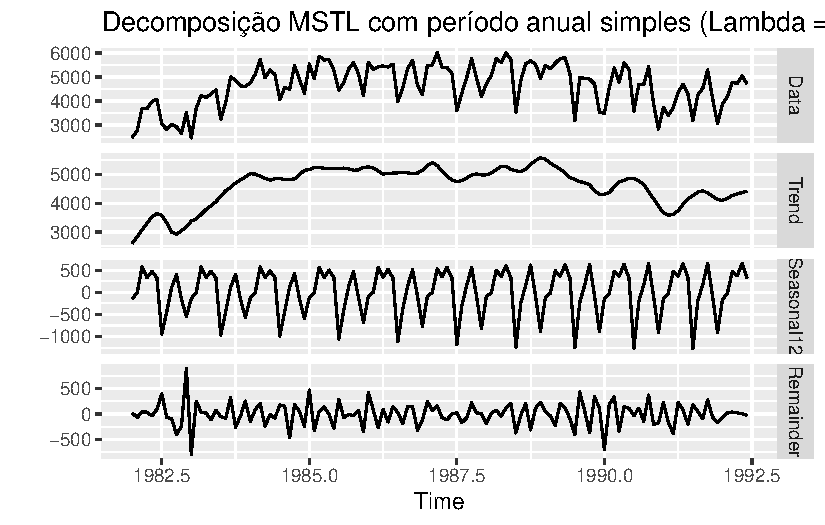
\includegraphics{T2_grupo10_files/figure-pdf/decomposicao-mstl-1.pdf}

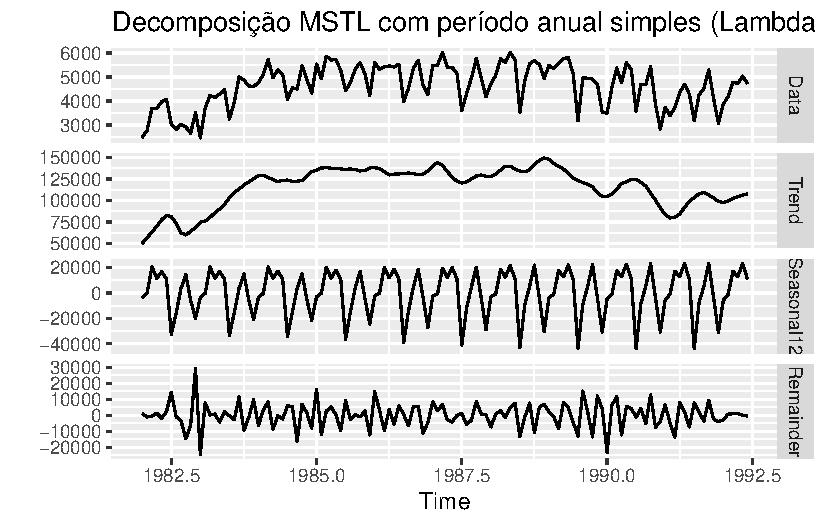
\includegraphics{T2_grupo10_files/figure-pdf/decomposicao-mstl-2.pdf}

Aplicando a decomposição MSTL com sazonalidade anual, é possível
visualizar uma tendência de crescimento no inicio das medições, passando
por uma estabilização e posterior decrescimento. Ao final, a série
parece retomar um pequeno crescimento. Além disso, é possível notar que
a série tem um componente sazonal mensal, com ciclos claros. Por fim, o
ruído parece se aproximar de um padãr de ruído branco.

\hypertarget{modelos-arima-seleuxe7uxe3o-transformauxe7uxf5es-e-resuxedduos}{%
\section{Modelos ARIMA: seleção, transformações e
resíduos}\label{modelos-arima-seleuxe7uxe3o-transformauxe7uxf5es-e-resuxedduos}}

\hypertarget{sem-transformauxe7uxe3o-de-box-cox}{%
\subsection{Sem transformação de
Box-Cox}\label{sem-transformauxe7uxe3o-de-box-cox}}

\begin{verbatim}

    KPSS Test for Level Stationarity

data:  serie_ms
KPSS Level = 0.52764, Truncation lag parameter = 4, p-value = 0.03544
\end{verbatim}

\begin{verbatim}
[1] 1
\end{verbatim}

\begin{verbatim}
[1] 1
\end{verbatim}

\begin{verbatim}

    KPSS Test for Level Stationarity

data:  serie_ms_diff
KPSS Level = 0.044309, Truncation lag parameter = 4, p-value = 0.1
\end{verbatim}

Inicialmente foi feito o teste de estacionaridade KPSS na série segundo
as hipóteses:

\begin{align}
  \begin{cases}
    H_0:\text{O processo é estacionário}\\
    H_1: \text{O processo possui raiz unitária}\\
  \end{cases}
\end{align}

O teste indica que a série não é estacionária (p-valor = 0,03544),
portanto, é necessário aplicar diferenciações para tornar a série
estacionária antes de ajustar um modelo adequado que se ajuste a série
em análise. O número de diferenciações simples necessárias é igual a um,
dessa forma, a estimativa para \emph{`d'} do modelo SARIMA é de
\emph{`d' = 1}. Além disso, em se tratanto de uma série sazonal, é
necessário verificar o número de diferenciações sazonais para retirar o
efeito da sazonalidade. Analogamente, foi obtido o valor de uma
diferenciação sazonal necessária, se tratando, portanto, do \emph{`D'}
do modelo SARIMA, sendo \emph{`D' = 1}. Para a diferenciação sazonal,
pelo ciclo sazonal ser igual a 12, é necessário a utilização do lag
sazonal igual a 12 (lag = 12).

\includegraphics{T2_grupo10_files/figure-pdf/grafico série diferenciada-1.pdf}

\begin{verbatim}

    KPSS Test for Level Stationarity

data:  serie_ms_diff
KPSS Level = 0.044309, Truncation lag parameter = 4, p-value = 0.1
\end{verbatim}

O gráfico acima mostra o comportamento da série após as diferenciações
simples e sazonal. A série aparenta ter comportamento estácionário, o
que foi confirmado a partir da aplicação do teste KPSS, cujas hipóteses
já foram explicitadas anteriormente. Por meio do teste foi possível
notar que a série realmente está estacionária após as diferenciações
(p-valor = 0,1), dessa forma, é possível proseguir com o procedimento de
seleção do modelo.

Para tal, se segue a análise dos gráficos ACF e PACF.

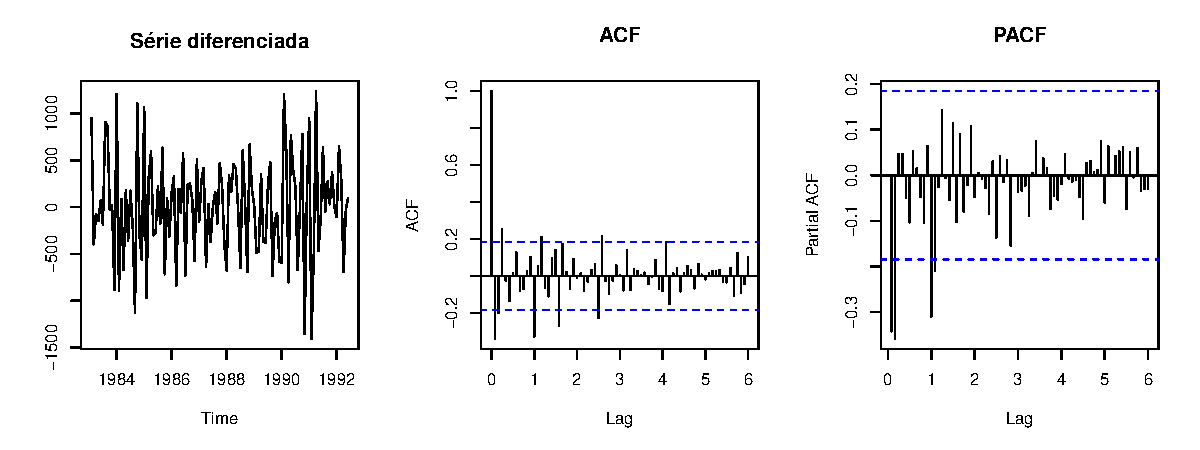
\includegraphics{T2_grupo10_files/figure-pdf/acf-pacf-sem-transformacao BoxCox-1.pdf}

É possível perceber que no ACF há uma quebra no primeiro lag simples, ao
passo que ocorre uma quebra no segundo lag do PACF. Porém, nenhum dos
gráficos apresenta comportamento bem definido, dificultando a
determinação do restante dos parâmetros do modelo SARIMA. Nesse
contexto, foi feito a combinação dos valores de \emph{p} e \emph{q},
entre 0 e 2, e de \emph{P} e \emph{Q}, nos valores 0 ou 1,
desconsiderando quando \emph{p} e \emph{q} fossem zero simultaneamente
e, analogamente, para \emph{P} e \emph{Q}. O melhor modelo, criado pelas
combinações de valores explicitados acima, foi selecionado segundo o
menor valor de AICc.

\begin{verbatim}
p = 0 , d = 1, q = 0 , P =  0 , D = 1, Q =  0 , AICc = 1750.899 
p = 0 , d = 1, q = 1 , P =  0 , D = 1, Q =  0 , AICc = 1729.316 
p = 0 , d = 1, q = 3 , P =  0 , D = 1, Q =  0 , AICc = 1729.225 
p = 1 , d = 1, q = 2 , P =  0 , D = 1, Q =  0 , AICc = 1729.027 
p = 2 , d = 1, q = 0 , P =  0 , D = 1, Q =  0 , AICc = 1724.938 
p = 0 , d = 1, q = 1 , P =  0 , D = 1, Q =  1 , AICc = 1709.211 
p = 2 , d = 1, q = 0 , P =  0 , D = 1, Q =  1 , AICc = 1706.182 
\end{verbatim}

\begin{verbatim}
[1] 1706.182
\end{verbatim}

A partir dos AICc, o modelo selecionado foi
\(SARIMA(2,1,0)(0,1,1)_{12}\), assim, pode-se prosseguir com a análise
dos resíduos.

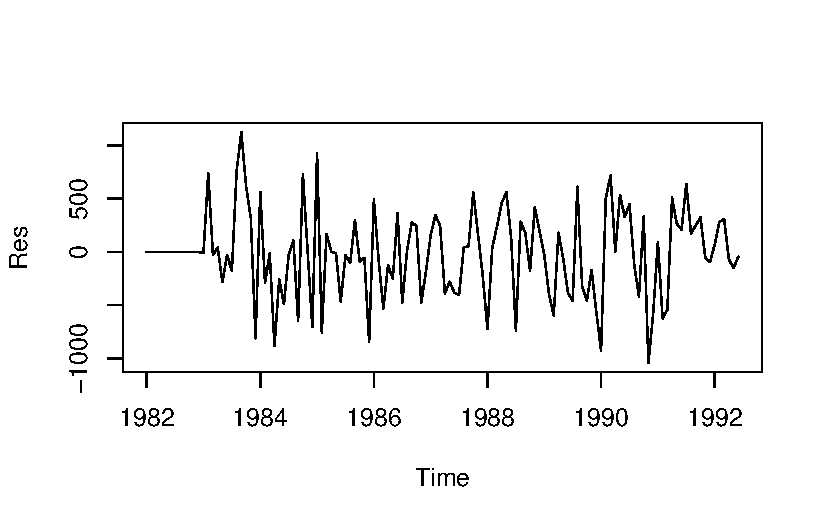
\includegraphics{T2_grupo10_files/figure-pdf/análise de resíduos - sem box-cox-1.pdf}

É notável que há uma sequência de resíduos iguais a zero no início da
série, e estes podem afetar as análises, dessa forma, os zeros foram
desconsiderados, sendo feita análise de resíduos de um ano após o início
da série, dados pela figura a seguir:

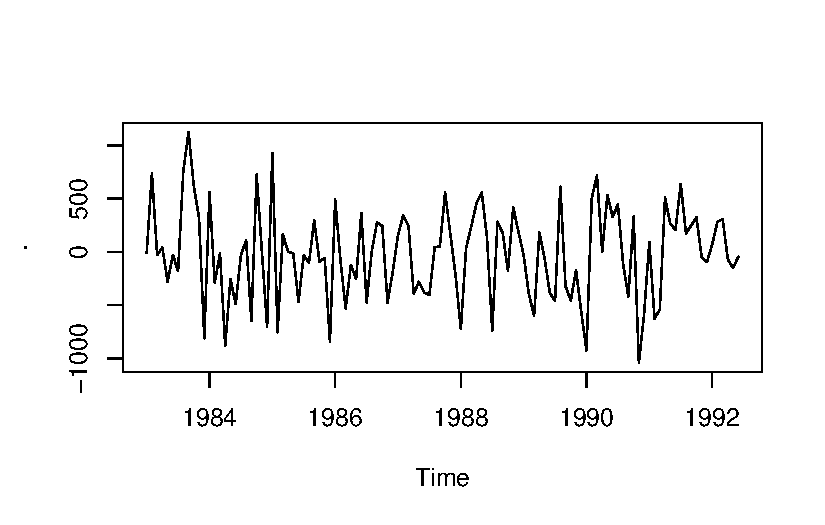
\includegraphics{T2_grupo10_files/figure-pdf/análise de resíduos - sem box-cox e sem zeros-1.pdf}

\begin{verbatim}

    KPSS Test for Level Stationarity

data:  E
KPSS Level = 0.062374, Truncation lag parameter = 4, p-value = 0.1
\end{verbatim}

Os resíduos aparentam ser estacionários, com média 0 e com variância
constante. Agora, foi testada a estacionariedade com um teste KPSS,
cujas as hipóteses já foram mencionadas. Como resultado, obtem-se que o
processo é estacionário (p-valor \textgreater{} 0, 1).

Além disso, a partir do gráfico do ACF, mostrado abaixo, pode-se
verificar a independência dos resíduos.

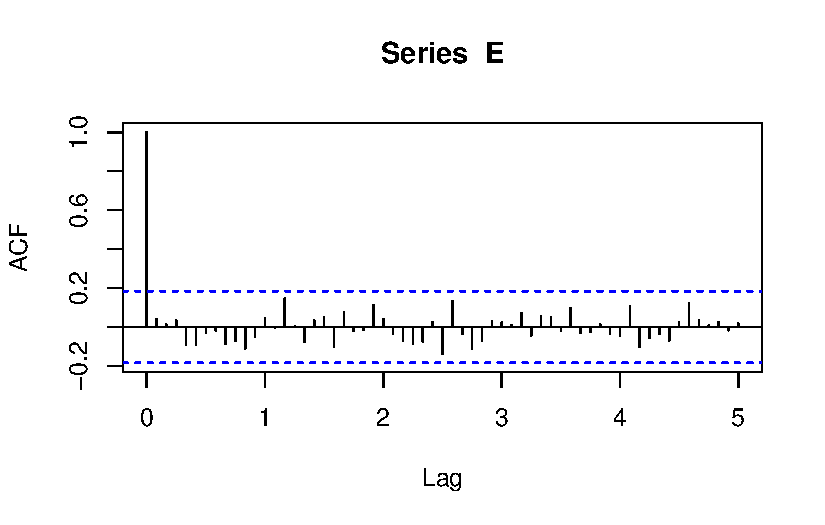
\includegraphics{T2_grupo10_files/figure-pdf/unnamed-chunk-1-1.pdf}

Observamos que praticamente todos os valores das autocorrelações não são
significantes, indicando a independência dos resíduos, o que necessita a
confirmação pelo teste de Ljung-Box, com base nas hipóteses:

\begin{align}
  \begin{cases}
    H_0:\text{Todas as correlações são iguais a zero}\\
    H_1: \text{Ao menos uma correlação é diferente de zero}\\
  \end{cases}
\end{align}

Assim, utilizando o teste com 20 graus de liberdade, obteve-se p-valor
de 0, 8923, e para 15, obteve-se 0, 8741, dessa maneira, utilizando o α
= 0, 05, não se rejeita H0, corroborando com a análise gráfica de que os
resíduos são independentes. Então, pode-se testar a normalidade,
primeiramente, por meio de uma representação gráfica.

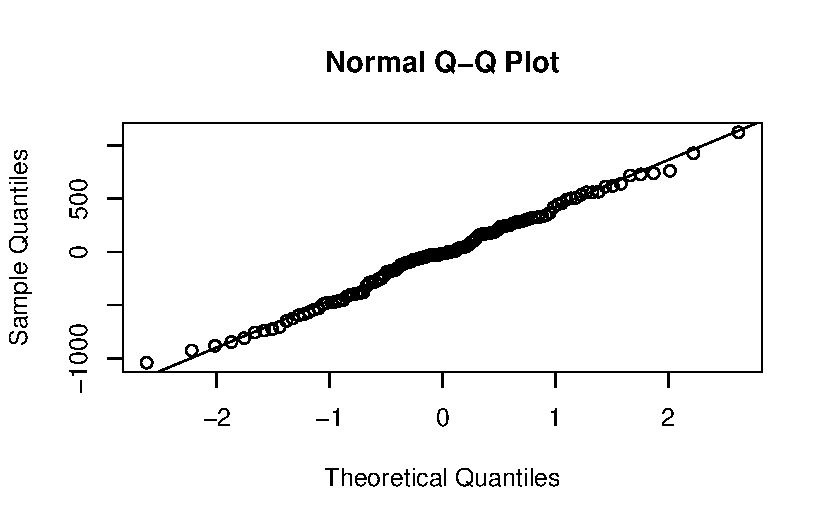
\includegraphics{T2_grupo10_files/figure-pdf/unnamed-chunk-2-1.pdf}

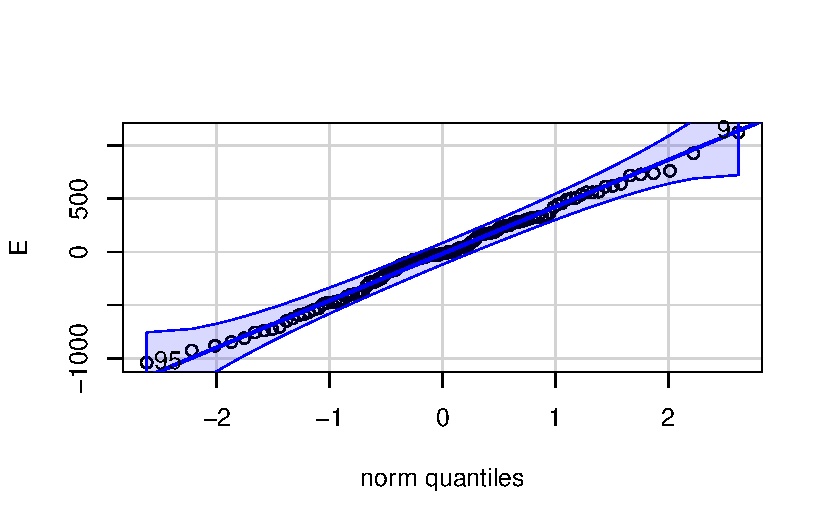
\includegraphics{T2_grupo10_files/figure-pdf/unnamed-chunk-2-2.pdf}

\begin{verbatim}
[1]  9 95
\end{verbatim}

\begin{verbatim}

    Shapiro-Wilk normality test

data:  E
W = 0.99331, p-value = 0.8598
\end{verbatim}

\begin{verbatim}

    Box-Ljung test

data:  E
X-squared = 12.639, df = 20, p-value = 0.8923
\end{verbatim}

\begin{verbatim}
       ar1        ar2       sma1 
-0.5096443 -0.3354277 -0.5080884 
\end{verbatim}

\begin{verbatim}
[1] 189154.6
\end{verbatim}

Assim, pela imagem, com envelope de 95\%, é basicamente certa a
normalidade dos resíduos, para confirmar, é conduzido o teste de
Shapiro-Wilk, sob hipóteses:

\begin{align}
  \begin{cases}
    H_0:\text{Os resíduos seguem distribuição normal}\\
    H_1: \text{Os resíduos não seguem distribuição normal}\\
  \end{cases}
\end{align}

Assim, com nível de significância de 0, 05, o teste de Shapiro-Wilk
confirma que os resíduos estão distribuidos segundo uma distribuição
normal.

\hypertarget{com-transformauxe7uxe3o-de-box-cox}{%
\subsection{Com transformação de
Box-Cox}\label{com-transformauxe7uxe3o-de-box-cox}}

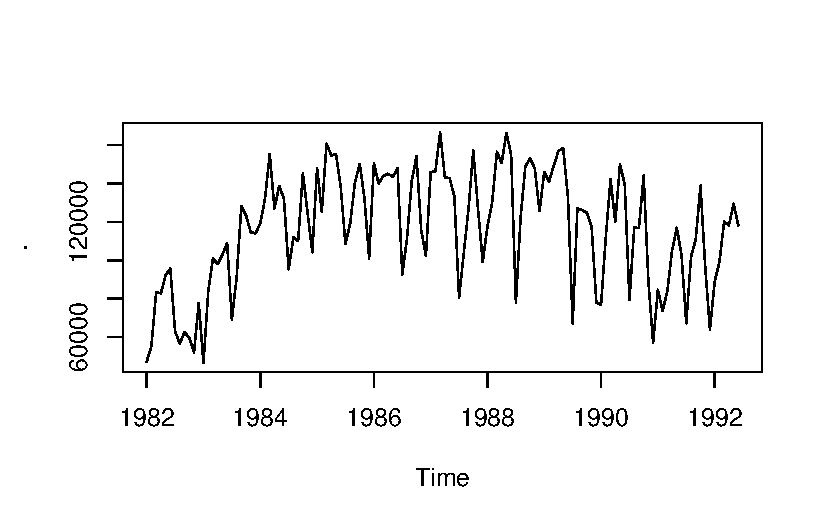
\includegraphics{T2_grupo10_files/figure-pdf/unnamed-chunk-3-1.pdf}

Percebe-se grande similaridade com a série original, e, pode-se
prosseguir da mesma maneira que anteriormente com o procedimento de
seleção. Primeiramente, testando a estacionariedade da série com o teste
KPSS a un nível de significância de 5\%, é possível concluir que a série
não é estacionária (p-valor = 0, 03658). Dessa maneira, analogamente à
análise da série sem a transformação Box-Cox, é necessário aplicar 1
diferenciação simples e de uma diferenciação sazonal para tornar a série
estácionária, sendo d = 1 e D = 1. Da mesma maneira que na análise
anterior, foi utilizado um sazonal de 12 para a diferenciação sazonal,
dessa maneira, a série diferenciada é a que se segue:

\begin{verbatim}

    KPSS Test for Level Stationarity

data:  x2
KPSS Level = 0.5226, Truncation lag parameter = 4, p-value = 0.03658
\end{verbatim}

\begin{verbatim}
[1] 1
\end{verbatim}

\begin{verbatim}
[1] 1
\end{verbatim}

\begin{verbatim}
Series: x2 
ARIMA(0,1,1)(0,1,1)[12] 

Coefficients:
          ma1     sma1
      -0.5166  -0.5532
s.e.   0.0825   0.1060

sigma^2 = 238912745:  log likelihood = -1251.65
AIC=2509.31   AICc=2509.53   BIC=2517.49
\end{verbatim}

\begin{verbatim}

    KPSS Test for Level Stationarity

data:  diff_bc
KPSS Level = 0.044088, Truncation lag parameter = 4, p-value = 0.1
\end{verbatim}

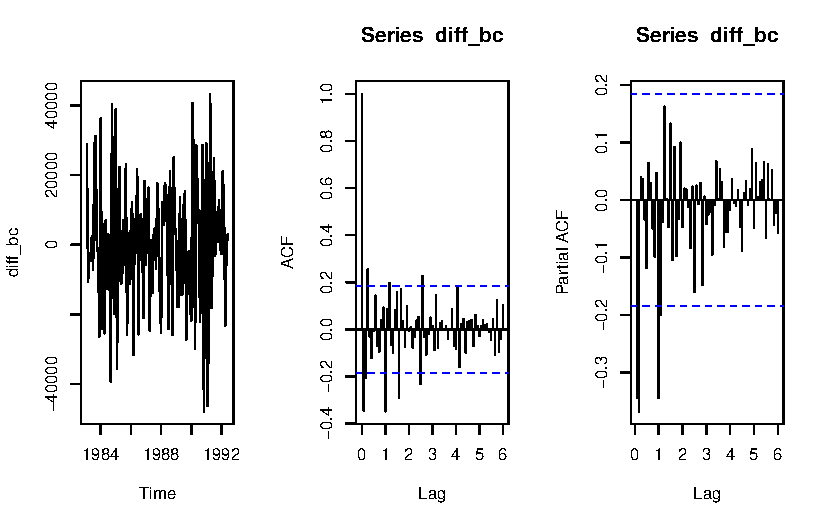
\includegraphics{T2_grupo10_files/figure-pdf/unnamed-chunk-5-1.pdf}

Assim ficou a série a partir de 1 diferenciação simples e sazonal.
Agora, analogamente à série sem transformação, é possível observar que a
série tem aparência estacionária, o que deve ser confirmado novamente a
partir do teste de KPSS de sob hipóteses já explicitadas. Assim, a
partir de um p-valor maior que 0.1, pôde-se confirmar que a série
diferenciada é estacionária e que é possível prosseguir com o
procedimento de seleção.

\begin{verbatim}
p = 0 , d = 1, q = 0 , P =  0 , D = 1, Q =  0 , AICc = 2553.741 
p = 0 , d = 1, q = 1 , P =  0 , D = 1, Q =  0 , AICc = 2531.436 
p = 0 , d = 1, q = 3 , P =  0 , D = 1, Q =  0 , AICc = 2531.137 
p = 1 , d = 1, q = 2 , P =  0 , D = 1, Q =  0 , AICc = 2530.789 
p = 2 , d = 1, q = 0 , P =  0 , D = 1, Q =  0 , AICc = 2526.922 
p = 0 , d = 1, q = 1 , P =  0 , D = 1, Q =  1 , AICc = 2509.529 
p = 2 , d = 1, q = 0 , P =  0 , D = 1, Q =  1 , AICc = 2506.5 
\end{verbatim}

\begin{verbatim}
[1] 2506.5
\end{verbatim}

Assim, pode-se observar comportamento similar ao da série sem a
transformação de Boxcox. Nesse sentido, no gráfico ACF há uma quebra no
primeiro lag simples, ao passo que há uma quebra no segundo lag no
gráfico PACF. Nenhum dos gráficos apresentou comportamento bem
definido.Para os lags sazonais, percebem-se valores significativos
apenas no primeiro lag, sendo assim, os valores de p e q serão testados
entre 0 e 2, já P e Q, nos valores 0 ou 1, desconsiderando quando p e q
forem 0 simultaneamente, e analogamente para P e Q. A partir dos AICc,
observou-se o melhor menor valor de 2506, 5 e assim, o modelo ajustado
foi um SARIMA\((2, 1, 0)(0, 1, 1)_{12}\), assim com no ajuste de modelo
sem utilização da transformação de Box-Cox.

Seguindo para análise dos resíduos, é possível observar que há uma
sequência de resíduos iguais a zero no início da série.

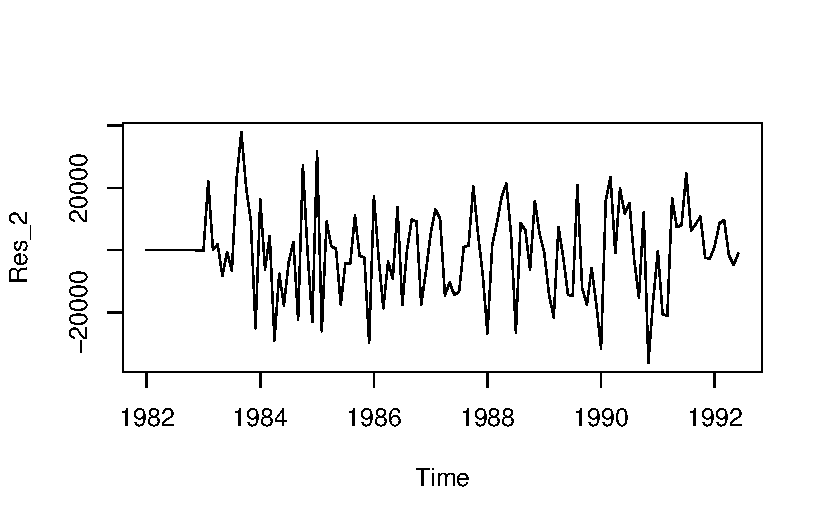
\includegraphics{T2_grupo10_files/figure-pdf/unnamed-chunk-7-1.pdf}

Assim, analogamente à série sem transformação, serão considerados apenas
os resíduos um ano após o início das observações, dados pela figura a
seguir:

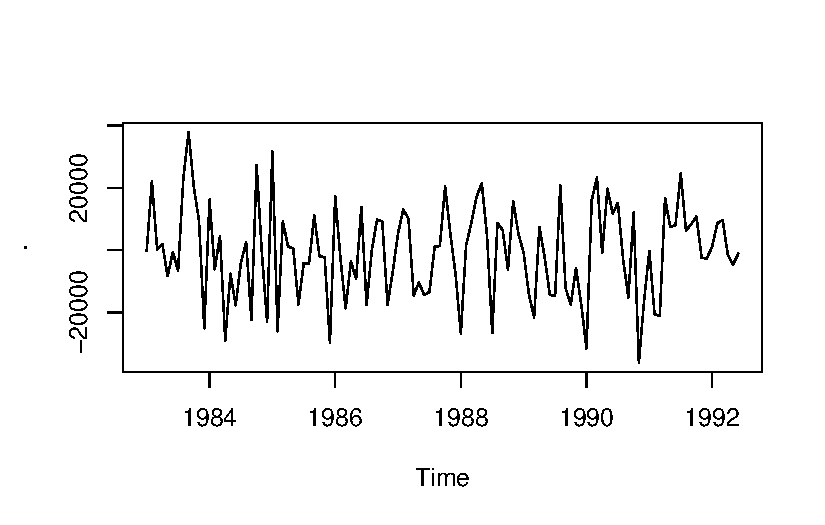
\includegraphics{T2_grupo10_files/figure-pdf/unnamed-chunk-8-1.pdf}

Agora, os residuos aparentam estacionariedade graficamente, mas para
testear realmente, utiliza-se o teste de KPSS. O teste mostra que os
resíduos são, de fato, estácionários (p-valor \textgreater{} 0, 1). Além
disso, pode-se visualizar pelo gráfico do ACF, a independência dos
resíduos:

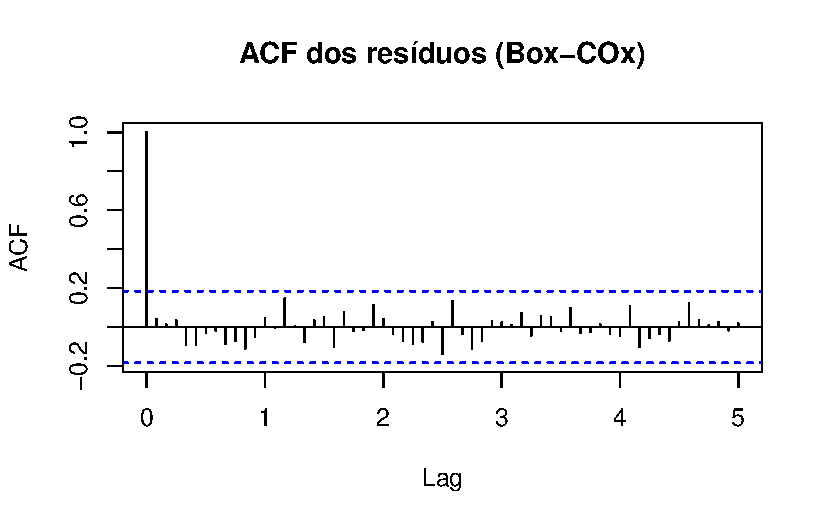
\includegraphics{T2_grupo10_files/figure-pdf/unnamed-chunk-9-1.pdf}

Assim, de maneira análoga à vista na série sem transformação de Box-Cox,
basicamente não há valores significativos, e, para realmente confirmar
independência, utiliza-se novamente o teste do tipo Ljung-Box. Assim,
com 20 graus de liberdade, o p-valor foi de 0, 86, e com 15 graus, o
p-valor resultou em 0.8443, portanto, para um nível de significância de
5\%, não se rejeita H0, indicando que a suspeita após a análise gráfica
estava correta, e os resíduos realmente são independentes. Por fim,
pode-se prosseguir com a análise da normalidade dos resíduos, por meio
da análise gráfica primeiramente.

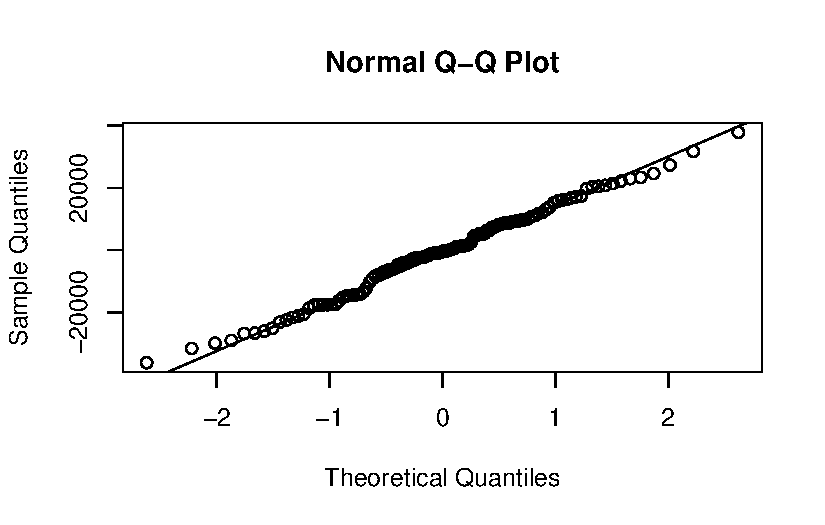
\includegraphics{T2_grupo10_files/figure-pdf/unnamed-chunk-10-1.pdf}

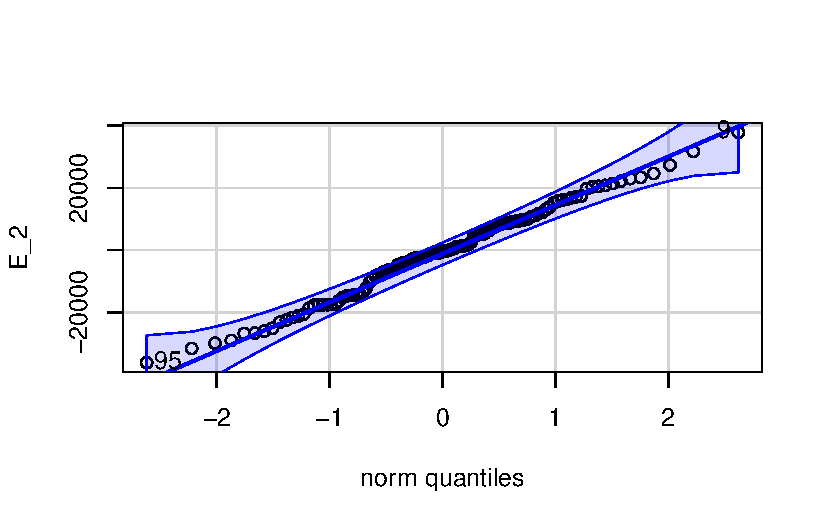
\includegraphics{T2_grupo10_files/figure-pdf/unnamed-chunk-10-2.pdf}

\begin{verbatim}
[1]  9 95
\end{verbatim}

\begin{verbatim}

    Shapiro-Wilk normality test

data:  E_2
W = 0.99199, p-value = 0.7513
\end{verbatim}

\begin{verbatim}

    KPSS Test for Level Stationarity

data:  E_2
KPSS Level = 0.062576, Truncation lag parameter = 4, p-value = 0.1
\end{verbatim}

\begin{verbatim}

    Box-Ljung test

data:  E_2
X-squared = 13.39, df = 20, p-value = 0.86
\end{verbatim}

\begin{verbatim}
       ar1        ar2       sma1 
-0.5059202 -0.3433980 -0.5264162 
\end{verbatim}

\begin{verbatim}
[1] 224602516
\end{verbatim}

A partir da análise gráfica, é possível observar indicação de
normalidade dos resíduos. Seguindo com o teste de Shapiro-Wilk, há
evidências de que os resíduos seguem distribuição normal (p-valor=0,
7513).

\hypertarget{modelos-ets-seleuxe7uxe3o-transformauxe7uxf5es-e-resuxedduos}{%
\section{Modelos ETS: seleção, transformações e
resíduos}\label{modelos-ets-seleuxe7uxe3o-transformauxe7uxf5es-e-resuxedduos}}

\begin{verbatim}
[1] 1
ETS(A,Ad,A) 

Call:
 ets(y = dados, model = model$modelo[i], damped = model$damp[i]) 

  Smoothing parameters:
    alpha = 0.46 
    beta  = 1e-04 
    gamma = 1e-04 
    phi   = 0.9628 

  Initial states:
    l = 2873.2425 
    b = 92.0764 
    s = -742.5204 -167.6501 488.8474 123.6439 -288.2857 -1061.117
           308.8648 564.7236 357.8395 543.2575 24.055 -151.6583

  sigma:  428.6046

     AIC     AICc      BIC 
2154.365 2160.757 2205.418 
[1] 2
ETS(A,A,A) 

Call:
 ets(y = dados, model = model$modelo[i], damped = model$damp[i]) 

  Smoothing parameters:
    alpha = 0.4973 
    beta  = 0.0149 
    gamma = 1e-04 

  Initial states:
    l = 2881.5847 
    b = 83.4981 
    s = -730.8711 -172.4496 489.9627 121.5461 -293.2277 -1060.087
           310.166 563.2084 359.0362 538.7735 26.4968 -152.5545

  sigma:  435.4436

     AIC     AICc      BIC 
2157.505 2163.171 2205.721 
[1] 3
[1] "Error in ets(dados, model = model$modelo[i], damped = model$damp[i]) : \n  Forbidden model combination\n"
attr(,"class")
[1] "try-error"
attr(,"condition")
<simpleError in ets(dados, model = model$modelo[i], damped = model$damp[i]): Forbidden model combination>
[1] 4
[1] "Error in ets(dados, model = model$modelo[i], damped = model$damp[i]) : \n  Forbidden model combination\n"
attr(,"class")
[1] "try-error"
attr(,"condition")
<simpleError in ets(dados, model = model$modelo[i], damped = model$damp[i]): Forbidden model combination>
[1] 5
ETS(A,Ad,N) 

Call:
 ets(y = dados, model = model$modelo[i], damped = model$damp[i]) 

  Smoothing parameters:
    alpha = 0.2022 
    beta  = 1e-04 
    phi   = 0.9711 

  Initial states:
    l = 3262.2671 
    b = 54.9193 

  sigma:  699.6524

     AIC     AICc      BIC 
2267.017 2267.723 2284.034 
[1] 6
ETS(A,A,N) 

Call:
 ets(y = dados, model = model$modelo[i], damped = model$damp[i]) 

  Smoothing parameters:
    alpha = 0.2561 
    beta  = 1e-04 

  Initial states:
    l = 3319.6533 
    b = 11.3537 

  sigma:  703.2468

     AIC     AICc      BIC 
2267.345 2267.845 2281.526 
[1] 7
[1] "Error in ets(dados, model = model$modelo[i], damped = model$damp[i]) : \n  Forbidden model combination\n"
attr(,"class")
[1] "try-error"
attr(,"condition")
<simpleError in ets(dados, model = model$modelo[i], damped = model$damp[i]): Forbidden model combination>
[1] 8
[1] "Error in ets(dados, model = model$modelo[i], damped = model$damp[i]) : \n  Forbidden model combination\n"
attr(,"class")
[1] "try-error"
attr(,"condition")
<simpleError in ets(dados, model = model$modelo[i], damped = model$damp[i]): Forbidden model combination>
[1] 9
[1] "Error in ets(dados, model = model$modelo[i], damped = model$damp[i]) : \n  Forbidden model combination\n"
attr(,"class")
[1] "try-error"
attr(,"condition")
<simpleError in ets(dados, model = model$modelo[i], damped = model$damp[i]): Forbidden model combination>
[1] 10
[1] "Error in ets(dados, model = model$modelo[i], damped = model$damp[i]) : \n  Forbidden model combination\n"
attr(,"class")
[1] "try-error"
attr(,"condition")
<simpleError in ets(dados, model = model$modelo[i], damped = model$damp[i]): Forbidden model combination>
[1] 11
[1] "Error in ets(dados, model = model$modelo[i], damped = model$damp[i]) : \n  Forbidden model combination\n"
attr(,"class")
[1] "try-error"
attr(,"condition")
<simpleError in ets(dados, model = model$modelo[i], damped = model$damp[i]): Forbidden model combination>
[1] 12
[1] "Error in ets(dados, model = model$modelo[i], damped = model$damp[i]) : \n  Forbidden model combination\n"
attr(,"class")
[1] "try-error"
attr(,"condition")
<simpleError in ets(dados, model = model$modelo[i], damped = model$damp[i]): Forbidden model combination>
[1] 13
[1] "Error in ets(dados, model = model$modelo[i], damped = model$damp[i]) : \n  Forbidden model combination\n"
attr(,"class")
[1] "try-error"
attr(,"condition")
<simpleError in ets(dados, model = model$modelo[i], damped = model$damp[i]): Forbidden model combination>
[1] 14
ETS(A,N,A) 

Call:
 ets(y = dados, model = model$modelo[i], damped = model$damp[i]) 

  Smoothing parameters:
    alpha = 0.5082 
    gamma = 1e-04 

  Initial states:
    l = 4021.6024 
    s = -739.9261 -173.8532 484.3761 131.9132 -289.0238 -1079.279
           320.7234 639.2768 334.7555 547.0071 16.7813 -192.7512

  sigma:  446.9512

     AIC     AICc      BIC 
2162.348 2166.712 2204.892 
[1] 15
[1] "Error in ets(dados, model = model$modelo[i], damped = model$damp[i]) : \n  Forbidden model combination\n"
attr(,"class")
[1] "try-error"
attr(,"condition")
<simpleError in ets(dados, model = model$modelo[i], damped = model$damp[i]): Forbidden model combination>
[1] 16
[1] "Error in ets(dados, model = model$modelo[i], damped = model$damp[i]) : \n  Forbidden model combination\n"
attr(,"class")
[1] "try-error"
attr(,"condition")
<simpleError in ets(dados, model = model$modelo[i], damped = model$damp[i]): Forbidden model combination>
[1] 17
[1] "Error in ets(dados, model = model$modelo[i], damped = model$damp[i]) : \n  Forbidden model combination\n"
attr(,"class")
[1] "try-error"
attr(,"condition")
<simpleError in ets(dados, model = model$modelo[i], damped = model$damp[i]): Forbidden model combination>
[1] 18
ETS(A,N,N) 

Call:
 ets(y = dados, model = model$modelo[i], damped = model$damp[i]) 

  Smoothing parameters:
    alpha = 0.2673 

  Initial states:
    l = 3135.6167 

  sigma:  698.2623

     AIC     AICc      BIC 
2263.601 2263.798 2272.110 
[1] 19
ETS(M,Ad,A) 

Call:
 ets(y = dados, model = model$modelo[i], damped = model$damp[i]) 

  Smoothing parameters:
    alpha = 0.2848 
    beta  = 1e-04 
    gamma = 1e-04 
    phi   = 0.9703 

  Initial states:
    l = 2865.1634 
    b = 94.8011 
    s = -741.5687 -168.7565 488.969 123.7533 -288.0692 -1055.661
           308.9004 564.5967 357.8223 543.1346 24.3001 -157.4208

  sigma:  0.1091

     AIC     AICc      BIC 
2194.143 2200.536 2245.197 
[1] 20
ETS(M,A,A) 

Call:
 ets(y = dados, model = model$modelo[i], damped = model$damp[i]) 

  Smoothing parameters:
    alpha = 0.3114 
    beta  = 0.0116 
    gamma = 1e-04 

  Initial states:
    l = 2884.0832 
    b = 93.0202 
    s = -693.2597 -165.8946 487.6633 180.0481 -292.417 -1047.902
           300.6935 552.5341 275.5544 542.2602 -1.1823 -138.0979

  sigma:  0.1098

     AIC     AICc      BIC 
2196.119 2201.786 2244.336 
[1] 21
ETS(M,Ad,M) 

Call:
 ets(y = dados, model = model$modelo[i], damped = model$damp[i]) 

  Smoothing parameters:
    alpha = 0.3659 
    beta  = 9e-04 
    gamma = 1e-04 
    phi   = 0.9768 

  Initial states:
    l = 2902.7456 
    b = 90.5988 
    s = 0.8623 0.9587 1.0966 1.02 0.9395 0.7798
           1.0788 1.1318 1.0769 1.1159 0.9953 0.9446

  sigma:  0.103

     AIC     AICc      BIC 
2179.418 2185.810 2230.471 
[1] 22
ETS(M,A,M) 

Call:
 ets(y = dados, model = model$modelo[i], damped = model$damp[i]) 

  Smoothing parameters:
    alpha = 0.3308 
    beta  = 0.0105 
    gamma = 1e-04 

  Initial states:
    l = 2908.8774 
    b = 83.9825 
    s = 0.8561 0.9567 1.0901 1.0216 0.9383 0.7799
           1.0936 1.1445 1.0914 1.1194 0.9845 0.924

  sigma:  0.1048

     AIC     AICc      BIC 
2184.055 2189.722 2232.272 
[1] 23
ETS(M,Ad,N) 

Call:
 ets(y = dados, model = model$modelo[i], damped = model$damp[i]) 

  Smoothing parameters:
    alpha = 0.2222 
    beta  = 1e-04 
    phi   = 0.9679 

  Initial states:
    l = 3263.0794 
    b = 78.9552 

  sigma:  0.1515

     AIC     AICc      BIC 
2267.284 2267.990 2284.302 
[1] 24
ETS(M,A,N) 

Call:
 ets(y = dados, model = model$modelo[i], damped = model$damp[i]) 

  Smoothing parameters:
    alpha = 0.3295 
    beta  = 0.0043 

  Initial states:
    l = 3262.7271 
    b = 72.8391 

  sigma:  0.1514

     AIC     AICc      BIC 
2269.144 2269.644 2283.325 
[1] 25
[1] "Error in ets(dados, model = model$modelo[i], damped = model$damp[i]) : \n  Forbidden model combination\n"
attr(,"class")
[1] "try-error"
attr(,"condition")
<simpleError in ets(dados, model = model$modelo[i], damped = model$damp[i]): Forbidden model combination>
[1] 26
[1] "Error in ets(dados, model = model$modelo[i], damped = model$damp[i]) : \n  Forbidden model combination\n"
attr(,"class")
[1] "try-error"
attr(,"condition")
<simpleError in ets(dados, model = model$modelo[i], damped = model$damp[i]): Forbidden model combination>
[1] 27
ETS(M,Md,M) 

Call:
 ets(y = dados, model = model$modelo[i], damped = model$damp[i]) 

  Smoothing parameters:
    alpha = 0.3705 
    beta  = 0.0045 
    gamma = 1e-04 
    phi   = 0.9698 

  Initial states:
    l = 2912.1767 
    b = 1.0349 
    s = 0.8469 0.9568 1.1026 1.0285 0.9386 0.7826
           1.0772 1.1308 1.0838 1.1176 0.9921 0.9424

  sigma:  0.1036

     AIC     AICc      BIC 
2181.290 2187.683 2232.343 
[1] 28
ETS(M,M,M) 

Call:
 ets(y = dados, model = model$modelo[i], damped = model$damp[i]) 

  Smoothing parameters:
    alpha = 0.5088 
    beta  = 0.016 
    gamma = 0.2117 

  Initial states:
    l = 2913.1548 
    b = 1.018 
    s = 0.9015 0.8722 1.0315 1.0343 0.9391 0.8241
           1.0926 1.0937 1.0985 1.1675 1.0174 0.9277

  sigma:  0.1086

     AIC     AICc      BIC 
2192.252 2197.918 2240.469 
[1] 29
ETS(M,Md,N) 

Call:
 ets(y = dados, model = model$modelo[i], damped = model$damp[i]) 

  Smoothing parameters:
    alpha = 0.2129 
    beta  = 1e-04 
    phi   = 0.958 

  Initial states:
    l = 3262.3304 
    b = 1.0242 

  sigma:  0.1518

     AIC     AICc      BIC 
2267.707 2268.413 2284.725 
[1] 30
ETS(M,M,N) 

Call:
 ets(y = dados, model = model$modelo[i], damped = model$damp[i]) 

  Smoothing parameters:
    alpha = 0.3019 
    beta  = 1e-04 

  Initial states:
    l = 3261.8504 
    b = 1.004 

  sigma:  0.1537

     AIC     AICc      BIC 
2268.625 2269.125 2282.806 
[1] 31
[1] "Error in ets(dados, model = model$modelo[i], damped = model$damp[i]) : \n  Forbidden model combination\n"
attr(,"class")
[1] "try-error"
attr(,"condition")
<simpleError in ets(dados, model = model$modelo[i], damped = model$damp[i]): Forbidden model combination>
[1] 32
ETS(M,N,A) 

Call:
 ets(y = dados, model = model$modelo[i], damped = model$damp[i]) 

  Smoothing parameters:
    alpha = 0.3794 
    gamma = 1e-04 

  Initial states:
    l = 4022.7944 
    s = -722.5848 -226.1109 480.6945 122.9523 -196.8044 -1055.387
           250.5592 656.0401 367.2533 563.3214 -43.8181 -196.1153

  sigma:  0.1216

     AIC     AICc      BIC 
2216.087 2220.451 2258.631 
[1] 33
[1] "Error in ets(dados, model = model$modelo[i], damped = model$damp[i]) : \n  Forbidden model combination\n"
attr(,"class")
[1] "try-error"
attr(,"condition")
<simpleError in ets(dados, model = model$modelo[i], damped = model$damp[i]): Forbidden model combination>
[1] 34
ETS(M,N,M) 

Call:
 ets(y = dados, model = model$modelo[i], damped = model$damp[i]) 

  Smoothing parameters:
    alpha = 0.3108 
    gamma = 0.0022 

  Initial states:
    l = 4061.2745 
    s = 0.8621 0.9501 1.1041 1.0246 0.9445 0.7811
           1.0861 1.1315 1.0851 1.1101 0.9928 0.9279

  sigma:  0.1124

     AIC     AICc      BIC 
2196.415 2200.778 2238.959 
[1] 35
[1] "Error in ets(dados, model = model$modelo[i], damped = model$damp[i]) : \n  Forbidden model combination\n"
attr(,"class")
[1] "try-error"
attr(,"condition")
<simpleError in ets(dados, model = model$modelo[i], damped = model$damp[i]): Forbidden model combination>
[1] 36
ETS(M,N,N) 

Call:
 ets(y = dados, model = model$modelo[i], damped = model$damp[i]) 

  Smoothing parameters:
    alpha = 0.3085 

  Initial states:
    l = 3191.2984 

  sigma:  0.1551

     AIC     AICc      BIC 
2265.474 2265.671 2273.983 
[1] 37
[1] "Error in ets(dados, model = model$modelo[i], damped = model$damp[i]) : \n  Invalid error type\n"
attr(,"class")
[1] "try-error"
attr(,"condition")
<simpleError in ets(dados, model = model$modelo[i], damped = model$damp[i]): Invalid error type>
[1] 38
[1] "Error in ets(dados, model = model$modelo[i], damped = model$damp[i]) : \n  Invalid error type\n"
attr(,"class")
[1] "try-error"
attr(,"condition")
<simpleError in ets(dados, model = model$modelo[i], damped = model$damp[i]): Invalid error type>
[1] 39
[1] "Error in ets(dados, model = model$modelo[i], damped = model$damp[i]) : \n  Invalid error type\n"
attr(,"class")
[1] "try-error"
attr(,"condition")
<simpleError in ets(dados, model = model$modelo[i], damped = model$damp[i]): Invalid error type>
[1] 40
[1] "Error in ets(dados, model = model$modelo[i], damped = model$damp[i]) : \n  Invalid error type\n"
attr(,"class")
[1] "try-error"
attr(,"condition")
<simpleError in ets(dados, model = model$modelo[i], damped = model$damp[i]): Invalid error type>
[1] 41
[1] "Error in ets(dados, model = model$modelo[i], damped = model$damp[i]) : \n  Invalid error type\n"
attr(,"class")
[1] "try-error"
attr(,"condition")
<simpleError in ets(dados, model = model$modelo[i], damped = model$damp[i]): Invalid error type>
[1] 42
[1] "Error in ets(dados, model = model$modelo[i], damped = model$damp[i]) : \n  Invalid error type\n"
attr(,"class")
[1] "try-error"
attr(,"condition")
<simpleError in ets(dados, model = model$modelo[i], damped = model$damp[i]): Invalid error type>
[1] 43
[1] "Error in ets(dados, model = model$modelo[i], damped = model$damp[i]) : \n  Invalid error type\n"
attr(,"class")
[1] "try-error"
attr(,"condition")
<simpleError in ets(dados, model = model$modelo[i], damped = model$damp[i]): Invalid error type>
[1] 44
[1] "Error in ets(dados, model = model$modelo[i], damped = model$damp[i]) : \n  Invalid error type\n"
attr(,"class")
[1] "try-error"
attr(,"condition")
<simpleError in ets(dados, model = model$modelo[i], damped = model$damp[i]): Invalid error type>
[1] 45
[1] "Error in ets(dados, model = model$modelo[i], damped = model$damp[i]) : \n  Invalid error type\n"
attr(,"class")
[1] "try-error"
attr(,"condition")
<simpleError in ets(dados, model = model$modelo[i], damped = model$damp[i]): Invalid error type>
[1] 46
[1] "Error in ets(dados, model = model$modelo[i], damped = model$damp[i]) : \n  Invalid error type\n"
attr(,"class")
[1] "try-error"
attr(,"condition")
<simpleError in ets(dados, model = model$modelo[i], damped = model$damp[i]): Invalid error type>
[1] 47
[1] "Error in ets(dados, model = model$modelo[i], damped = model$damp[i]) : \n  Invalid error type\n"
attr(,"class")
[1] "try-error"
attr(,"condition")
<simpleError in ets(dados, model = model$modelo[i], damped = model$damp[i]): Invalid error type>
[1] 48
[1] "Error in ets(dados, model = model$modelo[i], damped = model$damp[i]) : \n  Invalid error type\n"
attr(,"class")
[1] "try-error"
attr(,"condition")
<simpleError in ets(dados, model = model$modelo[i], damped = model$damp[i]): Invalid error type>
[1] 49
[1] "Error in ets(dados, model = model$modelo[i], damped = model$damp[i]) : \n  Invalid error type\n"
attr(,"class")
[1] "try-error"
attr(,"condition")
<simpleError in ets(dados, model = model$modelo[i], damped = model$damp[i]): Invalid error type>
[1] 50
[1] "Error in ets(dados, model = model$modelo[i], damped = model$damp[i]) : \n  Invalid error type\n"
attr(,"class")
[1] "try-error"
attr(,"condition")
<simpleError in ets(dados, model = model$modelo[i], damped = model$damp[i]): Invalid error type>
[1] 51
[1] "Error in ets(dados, model = model$modelo[i], damped = model$damp[i]) : \n  Invalid error type\n"
attr(,"class")
[1] "try-error"
attr(,"condition")
<simpleError in ets(dados, model = model$modelo[i], damped = model$damp[i]): Invalid error type>
[1] 52
[1] "Error in ets(dados, model = model$modelo[i], damped = model$damp[i]) : \n  Invalid error type\n"
attr(,"class")
[1] "try-error"
attr(,"condition")
<simpleError in ets(dados, model = model$modelo[i], damped = model$damp[i]): Invalid error type>
[1] 53
[1] "Error in ets(dados, model = model$modelo[i], damped = model$damp[i]) : \n  Invalid error type\n"
attr(,"class")
[1] "try-error"
attr(,"condition")
<simpleError in ets(dados, model = model$modelo[i], damped = model$damp[i]): Invalid error type>
[1] 54
[1] "Error in ets(dados, model = model$modelo[i], damped = model$damp[i]) : \n  Invalid error type\n"
attr(,"class")
[1] "try-error"
attr(,"condition")
<simpleError in ets(dados, model = model$modelo[i], damped = model$damp[i]): Invalid error type>
\end{verbatim}

\begin{longtable*}{lccc}
\toprule
Modelo & AIC & AICc & BIC\\
\midrule
\endfirsthead
\multicolumn{4}{@{}l}{\textit{(continued)}}\\
\toprule
Modelo & AIC & AICc & BIC\\
\midrule
\endhead

\endfoot
\bottomrule
\endlastfoot
\cellcolor{gray!15}{ETS(Ad,A,A)} & \cellcolor{gray!15}{2154.36} & \cellcolor{gray!15}{2160.76} & \cellcolor{gray!15}{2205.42}\\
ETS(A,A,A) & 2157.50 & 2163.17 & 2205.72\\
\cellcolor{gray!15}{ETS(A,N,A)} & \cellcolor{gray!15}{2162.35} & \cellcolor{gray!15}{2166.71} & \cellcolor{gray!15}{2204.89}\\
ETS(M,Ad,M) & 2179.42 & 2185.81 & 2230.47\\
\cellcolor{gray!15}{ETS(M,M,M)} & \cellcolor{gray!15}{2181.29} & \cellcolor{gray!15}{2187.68} & \cellcolor{gray!15}{2232.34}\\
ETS(M,A,M) & 2184.06 & 2189.72 & 2232.27\\
\cellcolor{gray!15}{ETS(M,M,M)} & \cellcolor{gray!15}{2192.25} & \cellcolor{gray!15}{2197.92} & \cellcolor{gray!15}{2240.47}\\
ETS(M,Ad,A) & 2194.14 & 2200.54 & 2245.20\\
\cellcolor{gray!15}{ETS(M,A,A)} & \cellcolor{gray!15}{2196.12} & \cellcolor{gray!15}{2201.79} & \cellcolor{gray!15}{2244.34}\\
ETS(M,N,M) & 2196.41 & 2200.78 & 2238.96\\*
\end{longtable*}

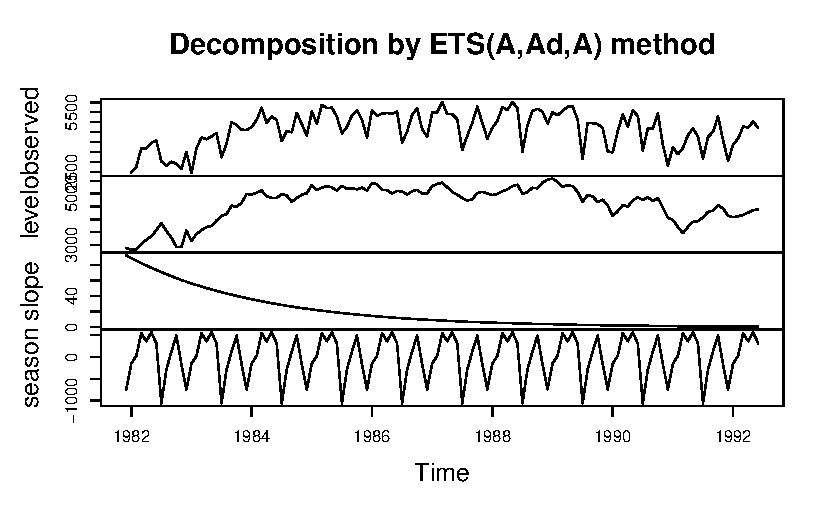
\includegraphics{T2_grupo10_files/figure-pdf/melhor-fit-ETL-sem-transf-1.pdf}

\hypertarget{resuxedduos}{%
\subsubsection{Resíduos}\label{resuxedduos}}

\hypertarget{modelo-com-transformauxe7uxe3o}{%
\subsection{Modelo com
transformação}\label{modelo-com-transformauxe7uxe3o}}

\hypertarget{seleuxe7uxe3o}{%
\subsubsection{Seleção}\label{seleuxe7uxe3o}}

a série com transformacao

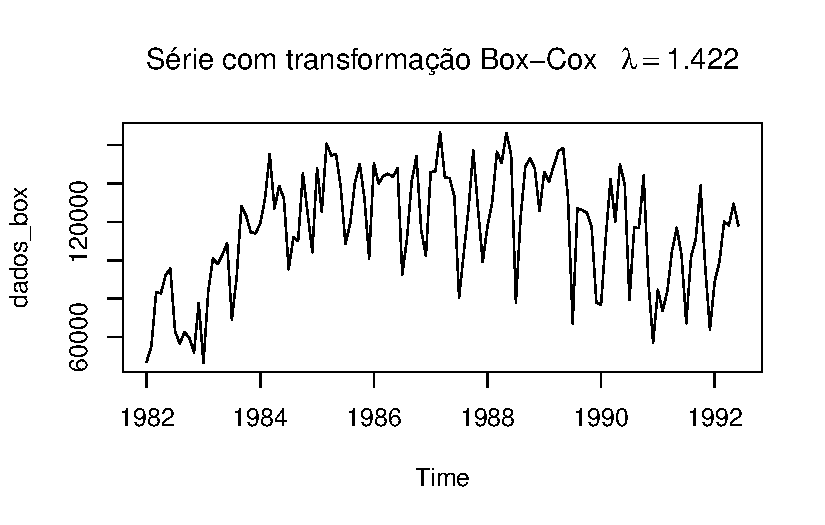
\includegraphics{T2_grupo10_files/figure-pdf/ETS-com-transf-1.pdf}

decomposicao

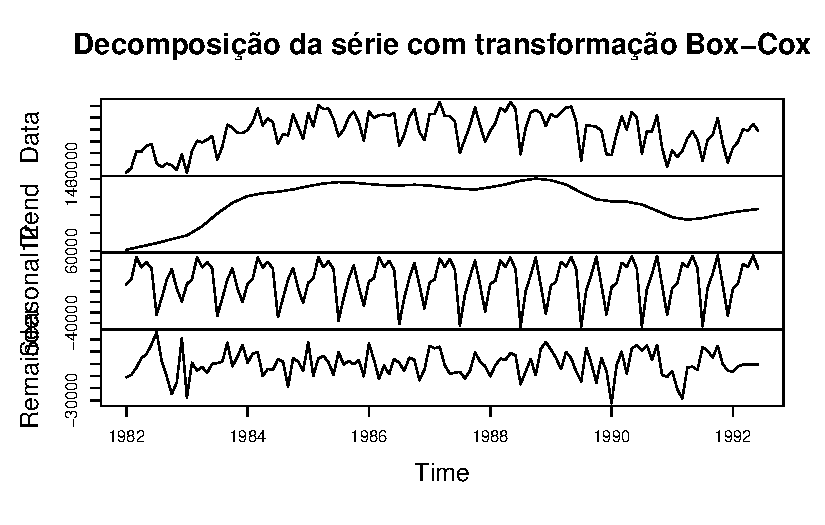
\includegraphics{T2_grupo10_files/figure-pdf/decomposicao-ets-com-transformacao-1.pdf}

selecao do modelo com transformação

\begin{longtable*}{lccc}
\toprule
Modelo transformado & AIC & AICc & BIC\\
\midrule
\endfirsthead
\multicolumn{4}{@{}l}{\textit{(continued)}}\\
\toprule
Modelo transformado & AIC & AICc & BIC\\
\midrule
\endhead

\endfoot
\bottomrule
\endlastfoot
\cellcolor{gray!15}{ETS(Ad,A,A)} & \cellcolor{gray!15}{2154.36} & \cellcolor{gray!15}{2160.76} & \cellcolor{gray!15}{2205.42}\\
ETS(A,A,A) & 2157.50 & 2163.17 & 2205.72\\
\cellcolor{gray!15}{ETS(A,N,A)} & \cellcolor{gray!15}{2162.35} & \cellcolor{gray!15}{2166.71} & \cellcolor{gray!15}{2204.89}\\
ETS(M,Ad,M) & 2179.42 & 2185.81 & 2230.47\\
\cellcolor{gray!15}{ETS(M,M,M)} & \cellcolor{gray!15}{2181.29} & \cellcolor{gray!15}{2187.68} & \cellcolor{gray!15}{2232.34}\\
ETS(M,A,M) & 2184.06 & 2189.72 & 2232.27\\
\cellcolor{gray!15}{ETS(M,M,M)} & \cellcolor{gray!15}{2192.25} & \cellcolor{gray!15}{2197.92} & \cellcolor{gray!15}{2240.47}\\
ETS(M,Ad,A) & 2194.14 & 2200.54 & 2245.20\\
\cellcolor{gray!15}{ETS(M,A,A)} & \cellcolor{gray!15}{2196.12} & \cellcolor{gray!15}{2201.79} & \cellcolor{gray!15}{2244.34}\\
ETS(M,N,M) & 2196.41 & 2200.78 & 2238.96\\*
\end{longtable*}

OS MODELOS SAO OS MESMO, PODEMO SELECIONAR O SEGUNDO MELHOR

\hypertarget{resuxedduos-1}{%
\subsubsection{Resíduos}\label{resuxedduos-1}}

\hypertarget{estudo-de-desempenho-preditivo}{%
\section{Estudo de desempenho
preditivo}\label{estudo-de-desempenho-preditivo}}

\hypertarget{resultados-da-janela-deslizante}{%
\subsection{Resultados da Janela
Deslizante}\label{resultados-da-janela-deslizante}}

\hypertarget{performance-em-relauxe7uxe3o-aos-horizontes-de-previsuxe3o}{%
\subsection{Performance em relação aos horizontes de
previsão}\label{performance-em-relauxe7uxe3o-aos-horizontes-de-previsuxe3o}}

\hypertarget{arima}{%
\subsubsection{ARIMA}\label{arima}}

\hypertarget{ets}{%
\subsubsection{ETS}\label{ets}}

\hypertarget{resultados}{%
\section{Resultados}\label{resultados}}

apresente em tabelas e gráficos as previsões dos 4 modelos selecionados
e também apresente em uma tabela os resultados de acurácia dos 4 modelos
selecionados e dos modelos benchmarks. Comente os resultados de modo
objetivo;

\hypertarget{apuxeandice}{%
\section{Apêndice}\label{apuxeandice}}

Todo o projeto de composição deste documento pode ser encontrado aqui:
https://github.com/cesar-galvao/trabalhos\_series



\end{document}
